\documentclass[11pt]{article}
\usepackage{tikz}
\usepackage{pgfmath}
\usepackage{setspace}
\usepackage{amsmath}
\usepackage{array}
\usepackage{hyperref}
\usepackage{enumerate}
\usepackage{enumitem}
\usepackage[normalem]{ulem}
\setlength{\pdfpageheight}{11in}
\setlength{\textheight}{9in}
\setlength{\voffset}{-1in}
\setlength{\oddsidemargin}{0pt}
\setlength{\marginparsep}{0pt}
\setlength{\marginparwidth}{0pt}
\setlength{\marginparpush}{0pt}
\setlength{\textwidth}{6.5in}

\pagestyle{empty}
%\setlength{}{}

\title{CSCE 515 Midterm Exam Prep}
\author{Brad Burkman}
\date{Last Edit: \today}

\begin{document}
\setlength{\parindent}{20pt}
\begin{spacing}{1.2}
\maketitle

\tableofcontents

%%%%%%%%%%%%%%%%%%
\section{Study Guide Questions}
%%%%%%%%%%%%%%%%%

\subsection{Question 1}
1.  Both raster and vector displays use a refresh buffer.  What is the difference between the two in terms of refresh buffer contents?

\subsection{First Punt, Brad Burkman, 11/17 7:41pm}

I have no idea.  I do not have a vector display refresh buffer in my notes, and I can't find it online.  

\

Here's what I do know.  

\

Raster displays have a bitmap of the color and intensity of each pixel.  Their refresh buffer holds the next screen to be displayed.  It may have two layers so that the swap between the displays doesn't happen in the middle of an update.  If it's a CRT monitor, it paints the pixels in rows, not following the contours of each object.  Raster displays have a constant refresh rate.  

\

Vector displays, like an oscilloscope, move a laser or electron beam over the screen following the contours of each object, drawing it smoothly.  It starts redrawing the screen after it has finished drawing the screen.  



\subsection{Question 2}
2.  For the midpoint line algorithm, how were floating point operations converted to integer operations for the main loop?  (Be as specific as possible.)

\subsubsection{First guess, Brad Burkman, 11/14 7:44pm}
The floating point operations were multiplied by [something like] the number of pixels that each integer represented, then rounded, because we don't care about being between two pixels; we have to pick one.  

\subsubsection{Second Atttempt, informed by notes, Brad Burkman, 11/14 7:58pm}
Since this sample question is about a small piece of the Besenham algorithm, I presume the actual exam question could be anything about it.  

\

Looking at the notes from 28 August, here's how the midpoint (Besenham) algorithm works.

\subsubsection{Midpoint Line (Besenham) Algorithm}

\begin{tikzpicture}[x=40mm, y=40mm]
	\draw (0,0) -- (4,1.6);
	\draw (0,0) circle (5pt);
	\draw (1,0) circle (5pt);
	\draw (2,1) circle (5pt);
	\draw (3,1) circle (5pt);
	\fill (0,0) circle (2pt) node [below] {$(x_0,y_0)$};
	\fill (1,0) circle (2pt) node [below] {$(x_{1},y_0)$};
	\path (1,-0.2) node [below] {$=(x_{0}+1,y_{0})$};
	\path (1,-0.4) node [below] {$=(x_{1},y_{1})$};
	\fill (1,1) circle (2pt) node [above] {$(x_{1},y_1)$};
	\fill (1,0.4) circle (2pt) node [left] {$(x_{1}, y_0+m) \ $};
	\fill (1,0.5) circle (2pt) node [above left] {$(x_{1}, y_0+0.5) \ $};
	\fill (2,0) circle (2pt) node [below] {$(x_{2},y_{1})$};
	\fill (2,0.4) circle (2pt) node [below right] {$(x_{2},y_{0}+m)$};
	\fill (2,0.5) circle (2pt) node [above right] {$(x_{2}, y_0+0.5)$};
	\fill (2,0.8) circle (2pt) node [right] {$(x_{2},y_{0}+2m)$};
	\fill (2,1) circle (2pt) node [above] {$(x_{2},y_{0}+1)$};
	\path (2,1.2) node [above] {$=(x_{2},y_{2})$};
	\fill (3,1) circle (2pt) node [below right] {$(x_3,y_2)= (x_0+3,y_0+1)$};
	\fill (3,1.2) circle (2pt) node [right] {$(x_0+3,y_0+3m)$};
	\fill (3,1.5) circle (2pt) node [right] {$(x_0+3,y_0+1.5)$};
	\fill (3,2) circle (2pt) node [right] {$(x_0+3,y_0+2)$};
\end{tikzpicture}  

Initialize $d$ at $m - 0.5$.  

Since in this case $d$ is negative, choose to move E rather than NE.  

At the second step, because we moved E, $d = d+m$, so $d = 2m - 0.5$.  

Since $d$ is positive, move NE.  

Now since we moved NE, $d = d+m-1 = (2m-0.5) + m - 1 = 3m - 1.5$

Since $d = 3m-1.5$ is negative, move E.

\subsubsection{Making it Faster}

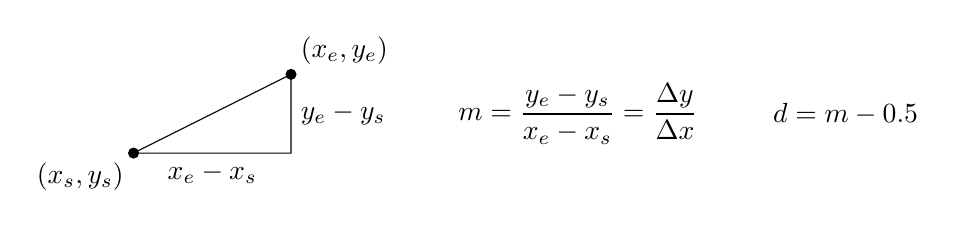
\begin{tikzpicture}[x=10mm,y=10mm]
	\draw (0,0) -- (2,1) -- (2,0) -- (0,0);
	\fill (0,0) circle (2pt) node [below left] {$(x_s,y_s)$};
	\fill (2,1) circle(2pt) node [above right] {$(x_e,y_e)$};
	\path (1,0) node [below] {$x_e-x_s$};
	\path (2,0.5) node [right] {$y_e - y_s$};
	\path (4,0.5) node [right] {$\displaystyle m = \frac{y_e - y_s}{x_e - x_s} = \frac{\Delta y}{\Delta x}$};
	\path (8,0.5) node [right] {$d = m-0.5$};
\end{tikzpicture}

Scale everything by $2 \Delta x$, so that $m = 2\Delta y$ and $d = 2\Delta y - \Delta x$.

\

Same example as above:

\begin{tikzpicture}[x=10mm,y=10mm]
	\draw (0,0) -- (5,2) -- (5,0) -- (0,0);
	\fill (0,0) circle (2pt) node [below left] {$(0,0)$};
	\fill (5,2) circle(2pt) node [above right] {$(5,2)$};
	\path (2.5,0) node [below] {$5$};
	\path (5,1) node [right] {$2$};
	\path (7,1) node [right] {$\displaystyle m = \frac{2}{5} = \frac{\Delta y}{\Delta x}$};
	\path (10,1) node [right] {$d = m-0.5$};
	\foreach \i in {0,1,2,3,4,5}{
		\draw [ultra thin, dashed] (\i,-1) -- (\i,3);
	}
\end{tikzpicture}

\

\begin{tikzpicture}[x=10mm,y=10mm]
	\draw (0,0) -- (5,2) -- (5,0) -- (0,0);
	\fill (0,0) circle (2pt) node [below left] {$(0,0)$};
	\fill (5,2) circle(2pt) node [above right] {$(50,20)$};
	\path (2.5,0) node [below] {$50$};
	\path (5,1) node [right] {$20$};
	\path (7,1) node [right] {$\displaystyle 2m\Delta x = 4 = \Delta y$};
	\path (7,0) node [right] {$d = 4-5 = -1$};
	\foreach \i in {0,1,2,3,4,5}{
		\draw [ultra thin, dashed] (\i,-1) -- (\i,3);
	}
\end{tikzpicture}

Initialize $d$ at $2\Delta y - \Delta x = 4-5 = -1$  

Since in this case $d$ is negative, choose to move E rather than NE.  

At the second step, because we moved E, $d = d+2\Delta y$, so $d = -1 + 4 = 3$.  

Since $d$ is positive, move NE.  

Now since we moved NE, $d = d+2 \Delta y - 10 = 3 + 2(2) - 10 = -3$

Since $d = -3$ is negative, move E.



\subsection{Question 3}
3.  What is meant by each of the three terms geometry, topology, and attributes for a polygonal surface model?

\subsubsection{Information from Class Notes, Brad Burkman, 17 November 10:11pm}

\begin{itemize}
	\item Vertex list gives the geometry, the shape.  
	\item Index list gives the topology, the relationships between neighbors.  
	\item Attributes are colors and normal vectors, perhaps the texture?
\end{itemize}

\subsection{Question 4}

\sout{4.  Give an example of an operation that would normally be faster with pointers-to-a-vertex-list mesh representation than with an explicit representation.  Justify your answer.  }

Replace with:

Triangle Strips Question

\subsection{Question 5}
5.  Answer true or false for each item below.  

For transforms as discussed in class:

\begin{itemize}
	\item Any two rotations are commutative.
	\item Any two translations are commutative.
	\item The inverse of a rotation matrix is its transpose.  
	\item The inverse of a translation matrix is its transpose.  
	\item For any composite sequence of translations and rotations, there exists a single rotation and translation pair that would have the same net effect.  [Dr. Borst says it's true.]
\end{itemize}

\subsubsection{Rotation Matrices}

What do we know about rotation matrices?

\begin{itemize}
	\item Each row, and each column, is a unit vector, because we're not changing scale.
	\item The determinant of the matrix is 1.
	\item They are orthogonal; {\tt i.e.} $R^{-1} = R^T$.
\end{itemize}

\subsection{Questions 6 and 7}
6,7.  Given a $4 \times 4$ homogeneous transform (sixteen numbers) for describing an object's local coordinate system with respect to the world coordinate system such that:

\begin{itemize}
	\item The object's local origin is at world coordinate $(x,y,z) = (4,0,2)$,
	\item The object's local $x$-axis direction matches the world's $z$-axis direction, and 
	\item The object's local $z$-axis direction matches the world's $-x$ (negative $x$) direction, 
\end{itemize}

Give the inverse of the transform.  

\subsection{Question 8}
8.  The diagrams below show a house model.  Give $\hat{\mathbf{n}}$, the unit normal vector for the right side of the roof.  

\subsubsection{First guess for \#8, Brad Burkman, 7:58pm, 11 November}
$$\hat{\mathbf{n}} = 
\left[
\begin{array}{>{\displaystyle}c<{\vrule width 0pt height 24pt depth 8pt}}
	 \frac{\sqrt2}{2}\cr
	 \frac{\sqrt2}{2}\cr
	 0 
\end{array}
\right]
$$

\subsubsection{Dr. Borst's Discussion}

Create a coordinate system, make a triangle, and use the cross product to find the normal.  

\subsection{Question 9}
9.  Recall the plane diagram above.  Suppose plane orientation is stored as an $X-Z-Y$ fixed axis set $(\theta, \phi, \alpha)$, that is, three rotations about fixed world axes in the order $X$, $Z$, $Y$.  In terms of the composite rotation resulting from these three components and for arbitrary plane orientation:

\begin{enumerate}[label=\arabic*)]
	\item A small change in $\theta$ ($X$ amount) will always cause rotation about:
	
	local $x_p$ \qquad local $y_p$ \qquad local $z_p$ \qquad world $x$ \qquad world $y$ \qquad world $z$ \qquad NOTA
	\item A small change in $\phi$ ($Z$ amount) will always cause rotation about:
	
	local $x_p$ \qquad local $y_p$ \qquad local $z_p$ \qquad world $x$ \qquad world $y$ \qquad world $z$ \qquad NOTA
	
	\item A small change in $\alpha$ ($Y$ amount) will always cause rotation about:
	
	local $x_p$ \qquad local $y_p$ \qquad local $z_p$ \qquad world $x$ \qquad world $y$ \qquad world $z$ \qquad NOTA
	\item If each component rotation is expressed as a matrix and then all three are composed into a single rotation matrix, the multiplication order for this representation would be:
	
	$R_XR_ZR_Y$ \qquad
	$R_YR_ZR_X$ \qquad
	$R_XR_YR_Z$ \qquad
	$R_ZR_YR_X$ \qquad
	NOTA
\end{enumerate}

\subsection{Question 10}
10.  How could we convert an orientation expressed in a 3-angle set convention above to a single quaternion representing the same orientation?  Give a concise but accurate conceptual description.

\subsubsection{Dr. Borst's Answer}

``Convert each of the three components into a quaternion, and multiply them.'' [Dr. Borst]

$X-Z-Y$ fixed axis set is multiplied as $R_YR_ZR_X$.


\subsection{Question 11}
11.  The graph below represents the relationships between coordinate systems (objects, if you prefer) using notation from lecture.  Suppose $\{D\}$ is the camera's local frame in an OpenGL application.  When rendering an object having vertices described in frame $\{E\}$, what would the value of the modelview matrix be?

\subsubsection{First Guess, Brad Burkman, 8:26pm 14 November}

$$
	^D_CT \cdot 
	^C_AT \cdot 
	^A_BT \cdot 
	^B_ET = 
	\left( ^C_DT \right)^{-1} \cdot
	\left( ^A_CT \right)^{-1} \cdot
	^A_BT \cdot 
	^B_ET
	$$
	
\subsection{Question 12}
12.  Suppose, for the above diagram, we want to rotate frame $\{B\}$ by a rotation transform $R$ that is to act as a rotation described with respect to the  current $\{B\}$ frame.  How exactly should $R$ be applied to update one of the transforms in the graph?

\subsubsection{Dr. Borst's Answer}

$^A_BT$ gets modified.  Multiply by $R$ on the right to be a local change to $B$.  


\subsection{Question 13}
13.  Give any one of the perspective projection matrices, $M_{per}$ from the lecture slides.  

\subsection{Question 14}
14.  What is meant by a normalizing transform and what two substeps can be used to build the normalizing transform for the orthographic projection case described in lecture?  A good conceptual description is sufficient; exact transforms are not requested.

\subsubsection{Dr. Borst's Answer}

Normalizing transform takes a box in the view and transforms it to $[-1,1]\times [-1,1] \times [-1,1]$.  Transform the center to the origin and scale.  

\subsection{Question 15}
15.  In the OpenGL pipeline, after the modelview matrix is applied to a vertex, the result is that the vertex is described with respect to which coordinate system?

\subsection{Question 16}
16.  The six common parameters (near, far, left, $\dots$) of a perspective frustum description are coordinates describing the viewing volume with respect to which coordinate system?

\subsubsection{First Guess, Brad Burkman, 9:03pm 14 November}

Eye (camera) coordinate system.

\subsection{Question 17}
17.  Below, circle all correct answers for questions about the illumination equation from lecture.  

\begin{enumerate}[label=\arabic*)]
	\item Which of the following vectors is (are) used in computing the ambient lighting term?
	
	Direction to light \qquad Surface normal \qquad Direction to viewer \qquad None
	\item Which of the following vectors is (are) used in computing the diffuse lighting term?
	
	Direction to light \qquad Surface normal \qquad Direction to viewer \qquad None
	\item Which of the following vectors is (are) used in computing the specular lighting term?
		
	Direction to light \qquad Surface normal \qquad Direction to viewer \qquad None

\end{enumerate}

\subsection{Question 18}
18.  Describe why a triangle may look different with Phong shading than with Gouraud shading, and include a sketch of shaded triangles that illustrate the difference you discuss. 

\subsection{Question 19}
\sout{19.  Sketch a scene with two or three polygons for which the painter's algorithm would be insufficient for visible surface determination.  }

\subsection{Question 20}
20.  Consider scan conversion of the illustrated triangle.  Assume that scan conversion is done from the bottom up, that the triangle crosses several scan lines, and that the geometry matches the illustration.  

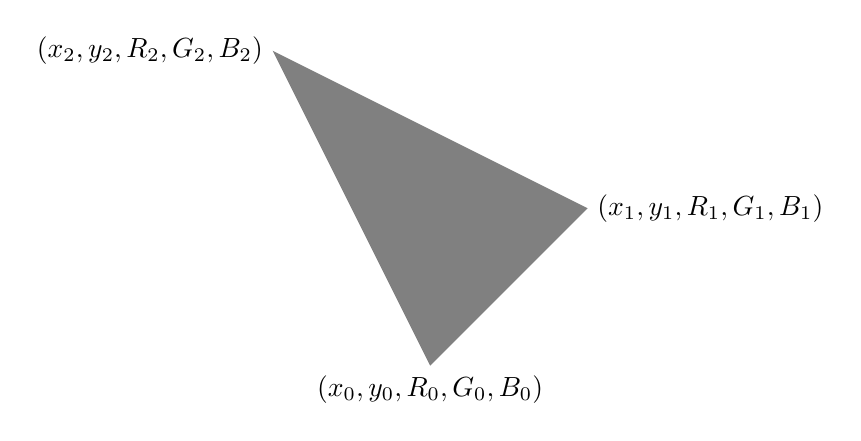
\begin{tikzpicture}[x=20mm,y=20mm]
	\coordinate (A) at (0,0);
	\coordinate (B) at (1,1);
	\coordinate (C) at (-1,2);
	\fill [gray] (A) -- (B) -- (C) -- (A);
	\path (A) node [below] {$(x_0, y_0, R_0, G_0, B_0)$};
	\path (B) node [right] {$(x_1,y_1,R_1,G_1,B_1)$};
	\path (C) node [left] {$(x_2,y_2,R_2,G_2,B_2)$};
\end{tikzpicture}

\begin{enumerate}[label=\arabic*)]
	\item In terms of the vertex coordinates and colors labeled on the diagram, give the coordinates and RGB color values for the first pixel to be colored.  
	\item In terms of the vertex coordinates and colors labeled on the diagram, give the coordinates and RGB values for the second pixel to be colored.  
\end{enumerate}

\subsubsection{First Guess, Brad Burkman, 9:23pm 14 November}

First pixel to be colored is the bottom.  
$$(x_0, y_0, R_0, G_0, B_0)$$

Second pixel to be colored is above left of that.  

$$m = \frac{y_2 - y_0}{x_2 - x_0} = \frac{\Delta y}{\Delta x}$$

Since we're going up one pixel, $\Delta y = 1$, so we're interested in $\Delta x$.  

$$\Delta x = \frac{x_2 - x_0}{y_2 - y_0}$$

and we're going to round it down, because we're talking about pixel values, which are integers.  

$$\Delta x = \left\lfloor\frac{x_2 - x_0}{y_2 - y_0}\right\rfloor$$

Change in colors works the same way.  

$$\Delta R = \frac{R_2 - R_0}{y_2 - y_0}$$

So the coordinates and colors of the second point to be colored are:

$$\left( x_0 + \left\lfloor\frac{x_2 - x_0}{y_2 - y_0}\right\rfloor, 
y_0 + 1, 
R_0 + \frac{R_2 - R_0}{y_2 - y_0},
G_0 + \frac{G_2 - G_0}{y_2 - y_0},
B_0 + \frac{B_2 - B_0}{y_2 - y_0}
\right)$$

\subsubsection{Dr. Borst's Discussion}

I realize I had forgotten about the offset between the line and the pixel.  

\end{spacing}
\end{document}

